%!TEX root = ../thesis.tex
%*******************************************************************************
%*********************************** First Chapter *****************************
%*******************************************************************************

\chapter{The Future of High Energy Physics }  %Title of the First Chapter

\ifpdf
    \graphicspath{{Introduction/Figs/Raster/}{Introduction/Figs/PDF/}{Introduction/Figs/}}
\else
    \graphicspath{{Introduction/Figs/Vector/}{Introduction/Figs/}}
\fi


%********************************** %First Section  **************************************
\section{Introduction} %Section - 1.1 

After the discovery of the Higgs boson, no physics beyond the standard model (SM)  - Fig.\ref{fig:StandardModel} - has been found at the Large Hadron Collider (LHC), which leads the search for light and weakly coupled long-lived particles.
FASER is a small and inexpensive detector installed in the far forward region of proton-proton ($pp$) collisions. It will collect data during Run 3 and probe new regions of the parameter space for new particles with masses in the 10 MeV to GeV range.
FASER requires no beam modifications and only requests luminosity  information. Further into the future, a larger
 FASER 2 will extend the sensitivity to even larger masses but will require significant civil engineering.


\begin{figure}[htbp!]
    \centering
    \begin{tikzpicture}[x=1.2cm, y=1.2cm]
      \draw[round] (-0.5,0.5) rectangle (4.4,-1.5);
      \draw[round] (-0.6,0.6) rectangle (5.0,-2.5);
      \draw[round] (-0.7,0.7) rectangle (5.6,-3.5);
    
      \node at(0, 0)   {\particle[gray!20!white]
                       {$u$}        {up}       {$2.3$ MeV}{1/2}{$2/3$}{R/G/B}};
      \node at(0,-1)   {\particle[gray!20!white]
                       {$d$}        {down}    {$4.8$ MeV}{1/2}{$-1/3$}{R/G/B}};
      \node at(0,-2)   {\particle[gray!20!white]
                       {$e$}        {electron}       {$511$ keV}{1/2}{$-1$}{}};
      \node at(0,-3)   {\particle[gray!20!white]
                       {$\nu_e$}    {$e$ neutrino}         {$<2$ eV}{1/2}{}{}};
      \node at(1, 0)   {\particle
                       {$c$}        {charm}   {$1.28$ GeV}{1/2}{$2/3$}{R/G/B}};
      \node at(1,-1)   {\particle 
                       {$s$}        {strange}  {$95$ MeV}{1/2}{$-1/3$}{R/G/B}};
      \node at(1,-2)   {\particle
                       {$\mu$}      {muon}         {$105.7$ MeV}{1/2}{$-1$}{}};
      \node at(1,-3)   {\particle
                       {$\nu_\mu$}  {$\mu$ neutrino}    {$<190$ keV}{1/2}{}{}};
      \node at(2, 0)   {\particle
                       {$t$}        {top}    {$173.2$ GeV}{1/2}{$2/3$}{R/G/B}};
      \node at(2,-1)   {\particle
                       {$b$}        {bottom}  {$4.7$ GeV}{1/2}{$-1/3$}{R/G/B}};
      \node at(2,-2)   {\particle
                       {$\tau$}     {tau}          {$1.777$ GeV}{1/2}{$-1$}{}};
      \node at(2,-3)   {\particle
                       {$\nu_\tau$} {$\tau$ neutrino}  {$<18.2$ MeV}{1/2}{}{}};
      \node at(3,-3)   {\particle[orange!20!white]
                       {$W^{\hspace{-.3ex}\scalebox{.5}{$\pm$}}$}
                                    {}              {$80.4$ GeV}{1}{$\pm1$}{}};
      \node at(4,-3)   {\particle[orange!20!white]
                       {$Z$}        {}                    {$91.2$ GeV}{1}{}{}};
      \node at(3.5,-2) {\particle[green!50!black!20]
                       {$\gamma$}   {photon}                        {}{1}{}{}};
      \node at(3.5,-1) {\particle[purple!20!white]
                       {$g$}        {gluon}                    {}{1}{}{color}};
      \node at(5,0)    {\particle[gray!50!white]
                       {$H$}        {Higgs}              {$125.1$ GeV}{0}{}{}};
      \node at(6.1,-3) {\particle
                       {}           {graviton}                       {}{}{}{}};
    
      \node at(4.25,-0.5) [force]      {strong nuclear force (color)};
      \node at(4.85,-1.5) [force]    {electromagnetic force (charge)};
      \node at(5.45,-2.4) [force] {weak nuclear force (weak isospin)};
      \node at(6.75,-2.5) [force]        {gravitational force (mass)};
    
      \draw [<-] (2.5,0.3)   -- (2.7,0.3)          node [legend] {charge};
      \draw [<-] (2.5,0.15)  -- (2.7,0.15)         node [legend] {colors};
      \draw [<-] (2.05,0.25) -- (2.3,0) -- (2.7,0) node [legend]   {mass};
      \draw [<-] (2.5,-0.3)  -- (2.7,-0.3)         node [legend]   {spin};
    
      \draw [mbrace] (-0.8,0.5)  -- (-0.8,-1.5)
                     node[leftlabel] {6 quarks\\(+6 anti-quarks)};
      \draw [mbrace] (-0.8,-1.5) -- (-0.8,-3.5)
                     node[leftlabel] {6 leptons\\(+6 anti-leptons)};
      \draw [mbrace] (-0.5,-3.6) -- (2.5,-3.6)
                     node[bottomlabel]
                     {12 fermions\\(+12 anti-fermions)\\increasing mass $\to$};
      \draw [mbrace] (2.5,-3.6) -- (5.5,-3.6)
                     node[bottomlabel] {5 bosons\\(+1 opposite charge $W$)};
    
      \draw [brace] (-0.5,.8) -- (0.5,.8) node[toplabel]         {standard matter};
      \draw [brace] (0.5,.8)  -- (2.5,.8) node[toplabel]         {unstable matter};
      \draw [brace] (2.5,.8)  -- (4.5,.8) node[toplabel]          {force carriers};
      \draw [brace] (4.5,.8)  -- (5.5,.8) node[toplabel]       {Goldstone\\bosons};
      \draw [brace] (5.5,.8)  -- (7,.8)   node[toplabel] {outside\\standard model};
    
      \node at (0,1.2)   [generation] {1\tiny st};
      \node at (1,1.2)   [generation] {2\tiny nd};
      \node at (2,1.2)   [generation] {3\tiny rd};
      \node at (2.8,1.2) [generation] {\tiny generation};
    \end{tikzpicture}
    \caption[Standard model of particle physics]{The standard model of particle physics. \cite{burgard_standard_nodate}}
    \label{fig:StandardModel}
\end{figure}


\section{How does FASER fit in the context of ATLAS and CMS}  %Section - 1.3 
\label{section1.3}

FASER (ForwArd Search ExpeRiment) is a proposed experiment dedicated to search for light and extremely weakly interacting particles at the LHC. It will be situated 480 m along the line-of-sight of the proton collisions in front of the ATLAS interaction point at the LHC. It has the prospect of discovering new particles such as dark photons, dark Higgs bosons, heavy neutral leptons and axion-like particles. FASER is part of the CERN's Physics Beyond Colliders study group which is an exploratory study aimed at exploiting the full scientific potential of CERN's accelerator complex and its scientific infrastructure through projects complementary to the existing LHC, HL-LHC and other possible future colliders.

\begin{wrapfigure}{R}{0.5\textwidth}
\centering    
    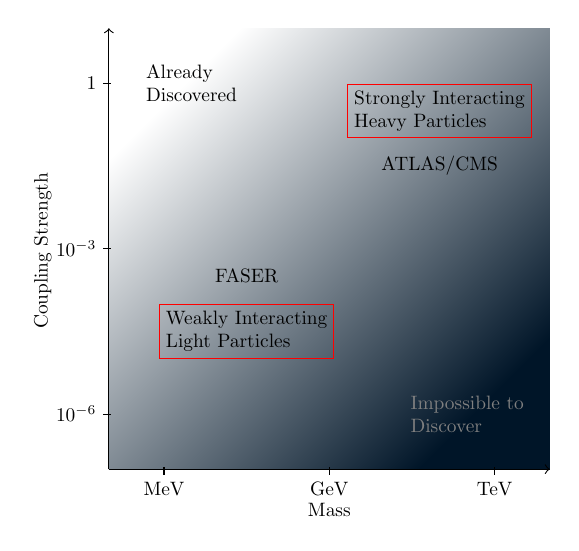
\begin{tikzpicture}[only marks,scale=0.7, every node/.style={scale=0.7}]
        \definecolor{deepblue} {HTML}{001528}
        \shade[top color=white,bottom color=deepblue, shading angle = 45] (0,0) rectangle (8,8);
        \node[draw=red, align=left] (wimp) at (2.5,2.5) {Weakly Interacting \\ Light Particles};
        \node[above of=wimp] {FASER};
        \node[align=left] at (1.5,7) {Already \\ Discovered};
        \node[draw=red, align=left] (sihp) at (6,6.5) {Strongly Interacting \\ Heavy Particles};
        \node[below of=sihp] {ATLAS/CMS};
        \node[align=left, text=gray] at (6.5,1) {Impossible to \\ Discover};
        \draw[->] (0,0) -- coordinate (x axis mid) (8,0);
        \draw[->] (0,0) -- coordinate (y axis mid) (0,8);
        \foreach \x/\xtext in {1/MeV,4/GeV,7/TeV}
            \draw (\x cm,1pt) -- (\x cm,-3pt) node[anchor=north] {\xtext};
        \foreach \y/\ytext in {1/10^{-6},4/10^{-3},7/1}
            \draw (1pt,\y cm) -- (-3pt,\y cm) node[anchor=east] {$\ytext$};
        \node[below=0.5cm] at (x axis mid) {Mass};
        \node[left=1.2cm,rotate=90,xshift=1.5cm] at (y axis mid) {Coupling Strength};
    \end{tikzpicture}    
\caption[Diagram coupling strenght vs Mass]{ATLAS and CMS focus on large transverse momentum ($p_{T}$) signatures that emerge in the roughly isotropic decay of such particles. There is a complementary class of viable new particles that are much lighter, with mass in the MeV to GeV range, much more weakly coupled to the SM.}
\label{fig:CouplingStrength_Mass}
\end{wrapfigure}

The four main LHC experiments that search for TeV-scale particles with high transverse momentum ($p_{T}$) may be misguided in the search for new particles. An area that isn't covered by these detectors, is the search for light particles with masses in the MeV to GeV range with low $p_{T}$. These new particles, that might be extremely weakly-coupled, may travel hundreds of meters without interacting with any material before decaying into known SM particles. During their travel, they would not be bent by magnets. Instead, they will continue along a straight line and only their decay products can be spotted by the FASER experiment. These hypothetical new particles would be long lived (LLP) and very collimated with the beam (of the order of the milliradian) allowing a small and inexpensive detector. For example, new particles that are produced in pion or B meson decays are typically produced within angles \[ \theta\sim\frac{\Lambda_{QCD}}{E}\sim\frac{m_{pion}}{E} \] of the beam collision axis, where E is the energy of the particle and $\Lambda_{QCD}$ is the scale of the pion mass. This implies that around 500 meters after the interaction point the downstream particle spread is 10 to 100 centimeters. \cite{faser_collaboration_letter_2018}

\newpage
\subsection{Beyond the Standard Model}

\begin{wrapfigure}{R}{0.25\textwidth}
  \centering
    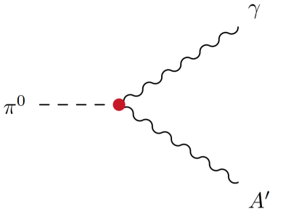
\includegraphics[width=0.24\textwidth]{DarkPhoton.png} 
    \caption[Neutral Pion Decay]{Neutral pion to dark photon decay.}
    \label{fig:Dark Photon}
\end{wrapfigure}

The FASER collaboration hopes to discover new particles through this experiment. An example for such a new particles is the dark photon, Fig.\ref{fig:Dark Photon}. Dark photons are hypothetical hidden sector (a collection of yet unobserved quantum fields) particles. Interaction between hidden sector and SM are weak, indirect and would be mediated via gravity or new particles. Dark photons are proposed as a force carrier, similar to the photon in the SM with a new abelian U(1) gauge symmetry. This new spin-1 gauge boson could couple very weakly to electrically charged particles through kinetic mixing with the normal photon. \cite{noauthor_dark_2019}
They could be produced in meson decays, where we see that the branching ratio (B) of the neutral pion to $A'$ and a photon is the same as the branching ratio for $\pi^0 \rightarrow \gamma\gamma$ but modified by the mass of  the $A'$:
\[
B(\pi^0 \rightarrow A'\gamma)=2\epsilon^2\left( 1-\frac{m^2_{A'}}{m^2_{\pi^0}} \right)^3B(\pi^0 \rightarrow \gamma\gamma)
\]

\begin{wrapfigure}{L}{0.28\textwidth}
  \centering
    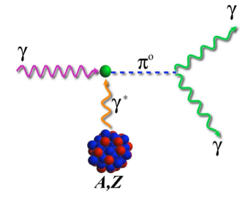
\includegraphics[width=0.26\textwidth]{Primakoff.png}
    \caption[Primakoff Effect]{The Primakoff effect is the resonant production of neutral pseudoscalar mesons by high-energy photons interacting with an atomic nucleus. \cite{kang_standard_1978}}
    \label{fig:Primakoff}
\end{wrapfigure}

Another type of new physics could be the discovery of axion-like-particles (ALPs). ALPs are hypothetical particles supposed stable, neutral and of very low mass (1 meV-$\mu$eV). They are a solution by Peccei-Quinn to the problem of CP violation in QCD.
There exists a possibility of using the LHC as a beam-dump experiment. Very high energy photons produced in the IP could interact with material in the Neutral Beam Absorbers (TAN, see Fig. \ref{fig:infrastructure}) and produce ALPs (~TeV energy) via Primakoff effect that could decay in FASER.



%********************************** % Nomenclature  *************************************
\nomenclature[z-PBC]{PBC}{Physics Beyond Colliders}
\nomenclature[z-CERN]{CERN}{Conseil Européen pour la Recherche Nucléaire}
\nomenclature[z-LHC]{LHC}{Large Hadron Collider}
\nomenclature[z-HL]{HL}{High Luminosity}
\nomenclature[z-ATLAS]{ATLAS}{A Toroidal LHC ApparatuS}
\nomenclature[z-eV]{eV}{Electronvolt}
\nomenclature[a-pt]{$p_{T}$}{Transverse Momentum}
\nomenclature[a-pp]{$pp$}{Proton-proton}
\nomenclature[z-SM]{SM}{Standard Model}
\nomenclature[z-IP]{IP}{Interaction Point}
\nomenclature[z-ALP]{ALP}{Axion like particles}
\nomenclature[z-CMS]{CMS}{Comact Muon Solenoid}